\section{Architechture of the REST API}
Before developing the code which creates the API endpoints, a proper architechture should be establish. 
Since it can be costly to backtrace and change central decisions made in this phase, a big amount of time have been spent thinking about the design. 
Most of this design was made by \textit{SW615F16} during sprint 1 and 2, but some refinements have been made by us during the resulutions of our tasks regarding the REST API. 
The full list of technologies used in the REST API and the development hereof will be listed in \myref{sec:techstack}, however in this section we will introduce the architecture used in the REST API. 

When we speak of the REST API were talking about the system which is located between the client and the database.
Its job is to serv content from the database to the client. 
\myref{fig:rest-architecture} contains a diagram which explains the basic layers of the architecture alongside the connections between said layers. 
The 3 layers depicted in the figure are: \textbf{Core}, \textbf{Persistance} and \textbf{Service}, the meaning of these are as follows:
\begin{description}
    \item[Core] \hfill \\
    The core layer contains the model of the REST API, a full class diagram will be shown later in \todo{ref her}.

    \item[Persistance] \hfill \\ 
    In the persistance layer we define and implement the data access objects (DAOs) which define how the objects in the database are accessed, as well as write and read files from the disk such as images. 
    Additionally we contstruct the tables for the relational database and some localdata which is used for unit tests and test data during development. 

    \item[Service] \hfill \\ 
    The service layer contains the code which is accessed by clients.
    Here we construct the endpoints which the clients can connect to; we use the DAOs in the persistance layer to access and manipulate data if the client is allowed to do so. 
\end{description}

\begin{figure}[h]
    \centering
    % 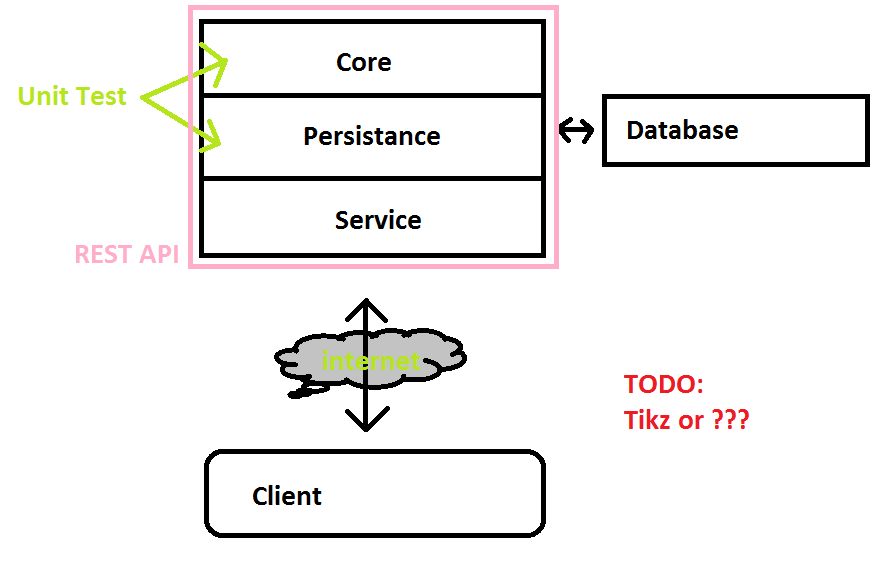
\includegraphics[width=0.8\textwidth]{figures/wip-stack.png}
    \pgfdeclarelayer{background}
\pgfdeclarelayer{foreground}
\pgfsetlayers{background,main,foreground}
\tikzstyle{double_arrow}=[latex'-latex']
\tikzstyle{component}=[draw, fill=blue!20, text width=8em,
text centered, minimum height=2.5em]
\tikzstyle{client_comp}=[draw, fill=blue!20, text width=4em,
text centered, minimum height=2.5em]
\begin{tikzpicture}[auto]
    % \node[component] (persistence) {Persistence};
    % \node[component, above = of persistence] (service) {Service};

    % \path (persistence.south -| persistence.east)+(1,0) node (core_a) {};
    % \path (service.north -| service.east)+(2,0) node (core_b) {};
    % \path[draw, fill = blue!20,] (core_a) rectangle (core_b);
    % \path ($ (core_a) !.5! (core_b) $) node {Core};

    % \path ($(persistence.west |- persistence.south) !.5! (core_b |- persistence.south)$) node (rest_buttom) {};
    % \path ($(service.west |- service.north) !.5! (core_b |- service.north)$) node (rest_top) {};

    % \node[component, below = 3cm of rest_buttom] (db) {Database --- MariaDB};
    % \node[draw, cloud, cloud puffs=8.9, cloud ignores aspect, minimum width=9em, minimum height=5em,fill=blue!20, above = 3cm of rest_top](web) {Internet};
    \node[component](core) {Core};
    \node[component, below = 0cm of core](persistence) {Persistence};
    \node[component, below = 0cm of persistence](service) {Service};
    \node[component, right = of persistence](db) {Database};
    \node[draw, cloud, cloud puffs=12, cloud ignores aspect, minimum width=9em, minimum height=5em,fill=blue!20, below = 0.8cm of service](web) {Internet};
    \node[client_comp, below = 1.5cm of web, anchor = west](client1) {$\text{Client}_{3}$};
    \node[client_comp, left = 0.2cm of client1](client2) {$\text{Client}_{2}$};
    \node[client_comp, left = 0.2cm of client2](client3) {$\text{Client}_{1}$};
    \node[right = 0.2cm of client1](client_dot){$\cdots$};
    \node[client_comp, right = 0.2cm of client_dot](client4) {$\text{Client}_{n}$};
    \begin{pgfonlayer}{background}
        % Compute a few helper coordinates
        \path (core.west |- core.north)+(-0.3,0.2) node (a) {};
        \node [above = 1mm of a, anchor = west]{REST API};
        \path (service.south -| service.east)+(+0.3,-0.2) node (b) {};
        \path[fill=green!20,rounded corners, draw=black!50, dashed]
        (a) rectangle (b);
    \end{pgfonlayer}

    \draw [double_arrow] (service) -- (web);
    \draw [double_arrow] (persistence) -- (db);
    \draw [double_arrow] (web) -- (client1.north);
    \draw [double_arrow] (web) -- (client2.north);
    \draw [double_arrow] (web) -- (client3.north);
    \draw [double_arrow] (web) -- (client4.north);
\end{tikzpicture}

    \caption{REST API architecture}
    \label{fig:rest-architecture}
\end{figure}

\todo[inline]{Maybe we should put some of the technologies we use directly in the figure?}

\subsection{Testing}
One of the benifits of seperating the REST API into the aforementioned layered architecture, is the ability to easily unit test the different components.
During the development we want to be able to test the REST API such that we can ensure whether or not the code works as intented. 
The Core and Persistance layers each have a test package which contains unit tests to ensure the correctness of the implementation. 
The tests in the persistance layer works as integration tests since it relies on the consistancy of the Core, the SQL which creates the database, and the DAOs.
With sufficient unit testing we can also easily do refactoring and change implementations details, meanwhile guarenteeing that the codes behaves as expected.
However one must comtemplate the false security which unit testing can give; the correctness of the code which is tested usign unit tests, heavily relies on the correctness of the tests themselves.
Because of the it is important that unit tests are relatively simple and unambigious, such that a programmer easily can comprehend whether or not the test itself is correct.
Moreover the code coverage of the unit tests is also an important factor, i.e. how many lines and effectively branches of the code is tested.
A codebase may have a dusin unit test which passed, but if only 50 \% of the code is tested, the unit tests cannot be used to conclude if the program behaves correctly.
Furthermore, it is important to keep in mind that testing only helps discover errors in a given piece of software, it cannot guarantee that there are no remaining faults in present. For more on software testing see Chapter 8 in \textit{Software Engineering (Tenth Edition)} By Ian Sommerville~\cite[Chapter~8]{SEBOOK}.

